% =====================================================================
%  RABBIT Bipedal Robot -- MATLAB Simulation & HZD Gait Framework
%  Technical documentation
%
%  Compile with:  pdflatex RABBIT_documentation.tex   (run twice for refs)
% =====================================================================
\documentclass[11pt,a4paper]{article}

\usepackage[utf8]{inputenc}
\usepackage[T1]{fontenc}
\usepackage{amsmath,amssymb}
\usepackage[margin=1in]{geometry}
\usepackage{booktabs}
\usepackage{longtable}
\usepackage{array}
\usepackage{xcolor}
\usepackage{listings}
\usepackage{tikz}
\usetikzlibrary{arrows.meta,positioning,fit,backgrounds}
\usepackage[hidelinks]{hyperref}

% ---- convenience macros --------------------------------------------
\newcommand{\code}[1]{\texttt{#1}}          % inline code (escape _ as \_)
\newcommand{\fname}[1]{\texttt{#1}}          % file name
\newcommand{\warn}[1]{\textcolor{red!70!black}{\textbf{#1}}}

\lstset{
  basicstyle=\ttfamily\small,
  breaklines=true,
  frame=single,
  columns=fullflexible,
  keepspaces=true,
  showstringspaces=false,
}

\newcolumntype{L}[1]{>{\raggedright\arraybackslash}p{#1}}

\title{\textbf{RABBIT Bipedal Robot}\\[2pt]
       \large A MATLAB Simulation and Hybrid Zero Dynamics Gait Framework\\[6pt]
       \normalsize Technical Documentation}
\author{Mohammad Malek}
\date{\today}

\begin{document}
\maketitle

\begin{abstract}
\noindent
This document describes a modular MATLAB framework for modeling, simulation,
control, and trajectory optimization of the RABBIT planar five--link
underactuated biped. The centrepiece is a working Hybrid Zero Dynamics (HZD)
gait--optimization pipeline that produces dynamically feasible, periodic walking
gaits and animates them. We cover the robot model, the continuous and hybrid
dynamics, the HZD control formulation, the nonlinear program solved with
\code{fmincon}, the software architecture and data flow, a per--folder file
reference, and reproducibility notes. Deviations between the documented and the
as--built code (broken legacy entry points, orphaned files) are flagged
explicitly.
\end{abstract}

%\tableofcontents
\bigskip

% =====================================================================
\section{Overview}
% =====================================================================
RABBIT is a planar, five--link, \emph{underactuated} biped: a torso plus two
legs, each with a hip and a knee. Walking is modelled as a hybrid dynamical
system --- continuous single--support (swing) dynamics punctuated by a discrete
impact when the swing foot strikes the ground. A gait is designed by imposing
\emph{virtual constraints} (B--spline reference trajectories for the actuated
joints) and choosing their coefficients, together with the periodic initial
state, so that the closed--loop system admits a stable periodic orbit while
minimizing actuator effort.

\paragraph{Dependencies.}
MATLAB with the \textbf{Symbolic Math Toolbox} (only to \emph{regenerate} the
dynamics; the generated files are committed) and the \textbf{Optimization
Toolbox} (\code{fmincon}, SQP --- required for the gait pipeline).

\paragraph{Working entry point.}
\begin{lstlisting}
startup                              % add all folders to the path
cd Trajectory_Optimization
rabbit_hzd_trajectory_optimization   % optimize one gait, inspect, animate
\end{lstlisting}
A gait library across walking speeds is built with \fname{build\_gait\_library.m}.
See Section~\ref{sec:known} for legacy entry points that no longer run.

% =====================================================================
\section{Robot model}
% =====================================================================
The generalized coordinates (7 DOF) are
\begin{equation}
  q = \begin{bmatrix} p_x & p_z & q_t & q_1 & q_2 & q_3 & q_4 \end{bmatrix}^{\!\top},
  \qquad
  x = \begin{bmatrix} q \\ \dot q \end{bmatrix} \in \mathbb{R}^{14}.
\end{equation}

\begin{table}[h]
\centering
\begin{tabular}{@{}clc@{}}
\toprule
symbol & meaning & actuated \\
\midrule
$p_x, p_z$ & torso base position (world frame) & no \\
$q_t$      & torso pitch angle                 & no \\
$q_1, q_2$ & stance--leg hip, knee             & \textbf{yes} \\
$q_3, q_4$ & swing--leg hip, knee              & \textbf{yes} \\
\bottomrule
\end{tabular}
\caption{Generalized coordinates. Four actuators drive $q_1\dots q_4$; the
floating base $(p_x,p_z,q_t)$ is unactuated, giving one degree of
underactuation in single support.}
\end{table}

The input map (\fname{Dynamics/input\_matrix.m}) is the constant
\begin{equation}
  B = \begin{bmatrix} 0_{3\times 4} \\ I_{4} \end{bmatrix} \in \mathbb{R}^{7\times 4}.
\end{equation}

\paragraph{Physical parameters.}
There is no separate model/parameter file; the physical parameters are baked
into the symbolic derivation
(\fname{Dynamics/rabbit\_energy\_model\_generalized\_Lagrange.m}, nested
\code{Mass\_Properties}): torso $10\,$kg / $0.75\,$m; each leg link (thigh,
shank) $5\,$kg / $0.5\,$m; gravity $g = 9.8062\,\mathrm{m/s^2}$.

\paragraph{Sign convention (important).}
The world--frame $Z$ axis is \emph{up--positive} (ground $=0$, above ground
$>0$), but $p_z$ is stored \emph{down--positive} in the generalized
coordinates, so the world--frame hip height is $-p_z$. All kinematic helpers
(\code{P\_st}, \code{P\_sw}, \code{Tt}, \code{get\_body\_points}) return
world--frame, up--positive heights. Mixing the two conventions has historically
caused sign bugs.

% =====================================================================
\section{Continuous dynamics}
% =====================================================================
The unconstrained equations of motion are
\begin{equation}
  M(q)\,\ddot q + V(q,\dot q) + G(q) = B\,u,
  \label{eq:eom}
\end{equation}
with $M(q)$ the mass/inertia matrix (\fname{Dynamics/M.m}), $V(q,\dot q)$ the
Coriolis/centrifugal vector (\fname{Dynamics/V.m}, called as
\code{V([q;dq])}), and $G(q)$ the gravity vector (\fname{Dynamics/G.m}).

\paragraph{Single--support (constrained) dynamics.}
During swing the stance foot is pinned by the holonomic contact constraint
$p_{\mathrm{st}}(q)=\text{const}$, i.e. at the acceleration level
\begin{equation}
  J_{\mathrm{st}}(q)\,\ddot q + \dot J_{\mathrm{st}}\dot q = 0,
  \qquad J_{\mathrm{st}} = \frac{\partial p_{\mathrm{st}}}{\partial q}\in\mathbb{R}^{2\times 7}.
\end{equation}
\fname{Dynamics/rabbit\_constrained\_dynamics.m} solves the resulting
saddle--point (KKT) system for the accelerations and the contact wrench
$\lambda$:
\begin{equation}
  \begin{bmatrix} M & -J_{\mathrm{st}}^{\top} \\ J_{\mathrm{st}} & 0 \end{bmatrix}
  \begin{bmatrix} \ddot q \\ \lambda \end{bmatrix}
  =
  \begin{bmatrix} B u - V - G \\ -\dot J_{\mathrm{st}}\dot q \end{bmatrix}.
\end{equation}

% =====================================================================
\section{Hybrid model}
% =====================================================================
Position is continuous across impact; only velocity jumps.
\begin{itemize}
  \item \textbf{Guard / event} (\fname{Contact/rabbit\_impact\_event.m}): the
        swing--foot height $p_{\mathrm{sw},z}(q)$ crosses zero from above.
  \item \textbf{Impact map} (\fname{Contact/rabbit\_impact\_map.m}):
        momentum--conserving reset enforcing zero post--impact swing--foot
        velocity,
        \begin{equation}
          \begin{bmatrix} M & -J_{\mathrm{sw}}^{\top} \\ J_{\mathrm{sw}} & 0 \end{bmatrix}
          \begin{bmatrix} \dot q^{+} \\ \lambda \end{bmatrix}
          =
          \begin{bmatrix} M\,\dot q^{-} \\ 0 \end{bmatrix}.
        \end{equation}
  \item \textbf{Reset map} (\fname{Reset\_Map/rabbit\_reset\_map.m}): relabels
        stance/swing legs (\fname{relabel\_state.m}) and re--plants the new
        stance foot on the ground ($p_z \mathrel{+}= p_{\mathrm{st},z}$). The
        horizontal coordinate is intentionally not shifted, so the robot walks
        forward continuously in the world frame.
\end{itemize}

% =====================================================================
\section{Phase variable and Hybrid Zero Dynamics}
% =====================================================================
\paragraph{Phase variable (linear in $q$).}
The gait ``clock'' is the absolute stance--leg angle, \emph{linear} in $q$:
\begin{equation}
  \theta(q) = q_t + q_1 + \tfrac{1}{2}q_2 = c\,q,
  \qquad c = \begin{bmatrix} 0 & 0 & 1 & 1 & \tfrac12 & 0 & 0 \end{bmatrix}.
  \label{eq:theta}
\end{equation}
This is implemented in \fname{Controller/theta\_of\_q.m}; its gradient
$\partial\theta/\partial q = c$ is the constant returned by
\fname{Controller/dtheta\_dq\_of.m}. Because both leg links have length
$\tfrac12$, the geometric hip--to--foot angle $\operatorname{atan2}$ equals
\eqref{eq:theta} exactly for all physical poses ($|q_2|<\pi$); the linear form
is preferred because \emph{it cannot wrap at $\pm\pi$} and matches Westervelt's
Hypothesis HH6, on which the HZD decoupling analysis relies.

\paragraph{Virtual constraints.}
The normalized phase is
\begin{equation}
  s = \frac{\theta - \theta^{-}}{\theta^{+} - \theta^{-}} \in [0,1],
\end{equation}
where $\theta^{-}$ is the phase at step start and $\theta^{+}$
(\code{p.theta\_plus}) at touchdown. The four actuated joints track a clamped
cubic B--spline reference $y_d(s)$,
\begin{equation}
  y(q) = q_{4:7} - y_d(s), \qquad u = -K_p\,y - K_d\,\dot y,
\end{equation}
with $K_p=400$, $K_d=40$. The B--spline is evaluated by
\fname{bspline\_eval.m} (basis functions from \fname{BSpline.m} /
\fname{BSpline\_derivative.m}); the whole closed loop is assembled in
\fname{Dynamics/hzd\_closed\_loop\_ode.m}, whose augmented state
$\xi = [x;\,\text{torque cost}]$ integrates the running cost alongside the
dynamics.

% =====================================================================
\section{Trajectory optimization (the nonlinear program)}
% =====================================================================
\paragraph{Decision vector.}
\begin{equation}
  z = \begin{bmatrix} \operatorname{vec}(\text{coeffs}) \\ x_{\text{start}} \end{bmatrix}
    \in \mathbb{R}^{\,n_u n_c + 14} = \mathbb{R}^{38},
\end{equation}
with $n_u=4$ actuated outputs and $n_c=6$ control points each
(\fname{unpack\_z.m}).

\paragraph{Cost} (\fname{hzd\_cost.m}): squared torque per unit step length
(Westervelt eq.~6.43),
\begin{equation}
  J(z) = \frac{1}{L_{\text{step}}}\int_0^{T_{\text{step}}} \lVert u(t)\rVert_2^2\, dt,
\end{equation}
where $L_{\text{step}}$ is the stance--to--swing foot distance at impact.
Normalizing by $L_{\text{step}}$ removes the degenerate incentive to
``step in place''.

\paragraph{Constraints} (\fname{hzd\_constraints.m}). Equalities
($\mathrm{ceq}\in\mathbb{R}^{18}$):
\begin{itemize}
  \item one--step periodicity, $x_{\text{next}}(2\!:\!14) = x_{\text{start}}(2\!:\!14)$, with
        $x_{\text{next}} = \Delta_{\text{reset}}\!\big(\Delta_{\text{impact}}(x_{\text{end}})\big)$ \hfill (13);
  \item stance foot on ground at $t=0$ \hfill (1);
  \item stance foot zero velocity, $J_{\mathrm{st}}\dot q_{\text{start}}=0$ \hfill (2);
  \item touchdown phase, $\theta(q_{\text{end}}) = \theta^{+}$ \hfill (1);
  \item \textbf{NEC1} average walking rate, $L_{\text{step}}/T_{\text{step}} = v_{\text{des}}$ \hfill (1).
\end{itemize}
Inequalities ($c\in\mathbb{R}^{4}$, $c\le 0$): no ground penetration; mid--step
swing--foot clearance (NIC3); step--length floor; and orbital stability
(Section~\ref{sec:stability}, gated behind \code{p.enforce\_stability}).

\paragraph{Solver} (\fname{hzd\_problem\_setup.m}). \code{fmincon} SQP with
\emph{central} finite differences (the event--triggered \code{ode45} makes
forward differences noisy) and \code{ScaleProblem} \emph{off} (so reported
feasibility is directly comparable to the constraint tolerance). Cold starts
from $x_0$ are unreliable; \fname{build\_gait\_library.m} warm--starts each
speed from the previously converged gait and marches $v_{\text{des}}$ in small
steps.

\paragraph{Diagnostics.} \fname{inspect\_solution.m} prints and returns a full
breakdown of any $z$: the $\theta$ sweep, step length/duration, walking speed,
cost, every constraint residual, the worst violation, the within--step
stance--foot drift, and the orbital--stability radius $\rho$ (below).

% =====================================================================
\section{Orbital stability: periodic is not the same as stable}
\label{sec:stability}
% =====================================================================
This section is deliberately expanded for teaching, because it is the single
most instructive point in the pipeline.

\paragraph{The trap.} The periodicity equality makes $x_{\text{start}}$ a
\emph{fixed point} of the step--to--step (Poincar\'e) map
\begin{equation}
  x_{\text{next}} = P(x_{\text{start}})
      := \Delta_{\text{reset}}\big(\Delta_{\text{impact}}(\varphi_{\text{step}}(x_{\text{start}}))\big),
  \label{eq:poincare}
\end{equation}
where $\varphi_{\text{step}}$ is one closed--loop swing phase. But \emph{a fixed
point can be unstable.} Satisfying periodicity to machine precision guarantees a
limit cycle \emph{exists}; it says nothing about whether the robot stays on it.

\paragraph{The diagnosis.} Linearize \eqref{eq:poincare} about the fixed point,
$A = \partial P/\partial x$, and look at its spectral radius
\begin{equation}
  \rho = \max_i |\lambda_i(A)|.
\end{equation}
The gait is orbitally (asymptotically) stable iff $\rho < 1$. This is
Westervelt's stability requirement (informally, NEC5). For the reference seed
gait obtained by enforcing periodicity \emph{alone}, the numbers are stark:
\begin{center}
\begin{tabular}{@{}lll@{}}
\toprule
$\max|\text{periodicity}|$ & $\rho$ & open--loop $|\dot q|$ over 6 steps \\
\midrule
$0.007$ (excellent) & $\approx 3$ (unstable) &
  $6 \to 6 \to 19 \to 891 \to 949 \to 440$ \\
\bottomrule
\end{tabular}
\end{center}
The orbit is a near--perfect fixed point that the robot falls off after two
steps. Every downstream symptom we observed --- stance--foot drift growing
across a step, Baumgarte constraint stabilization diverging, the Poincar\'e
settling iteration blowing up, fragile speed continuation --- is the same
instability seen from a different angle: an orbit with $\rho>1$ amplifies
\emph{every} perturbation, numerical or physical.

\paragraph{The remedy.} Add $\rho < 1$ as an optimization constraint.
\fname{poincare\_stability.m} builds $A$ by central finite differences on the
13 periodic states (index $2\!:\!14$; $p_x$ is the translation gauge and is
excluded),
\begin{equation}
  A_{:,j} = \frac{P\!\left(x_{\text{start}} + h\,e_j\right) - P\!\left(x_{\text{start}} - h\,e_j\right)}{2h},
  \qquad j = 1,\dots,13,
\end{equation}
and returns $\rho = \max_i|\lambda_i(A)|$. \fname{hzd\_constraints.m} then adds
the inequality $\rho - \rho_{\max} \le 0$ (with $\rho_{\max}=0.95$).

\paragraph{Cost and workflow.} Each $\rho$ evaluation costs $\approx 2\times 13 =
26$ step simulations, and \code{fmincon} finite--differences the constraint over
$38$ variables --- hundreds to thousands of simulations per iteration. The
constraint is therefore \textbf{gated} behind \code{p.enforce\_stability}
(default \code{false}). The recommended workflow is two--phase:
\begin{enumerate}
  \item solve a \emph{periodic} gait with stability off (fast);
  \item turn \code{p.enforce\_stability = true} and re--solve
        \emph{warm--started} from that gait to drive $\rho$ below~1.
\end{enumerate}
\fname{inspect\_solution.m} reports $\rho$ on every call regardless of the gate,
so stability is always visible even when it is not being enforced.

\paragraph{Analogy.} Just as the \emph{step--length floor} was the missing
constraint that stopped the optimizer exploiting a degenerate ``step in place'',
the \emph{stability bound} is the missing constraint that stops it returning a
mathematically periodic but physically un--walkable orbit. In both cases the
optimizer was doing exactly what it was told; the specification was incomplete.

% =====================================================================
\section{Software architecture and data flow}
% =====================================================================
\begin{figure}[h]
\centering
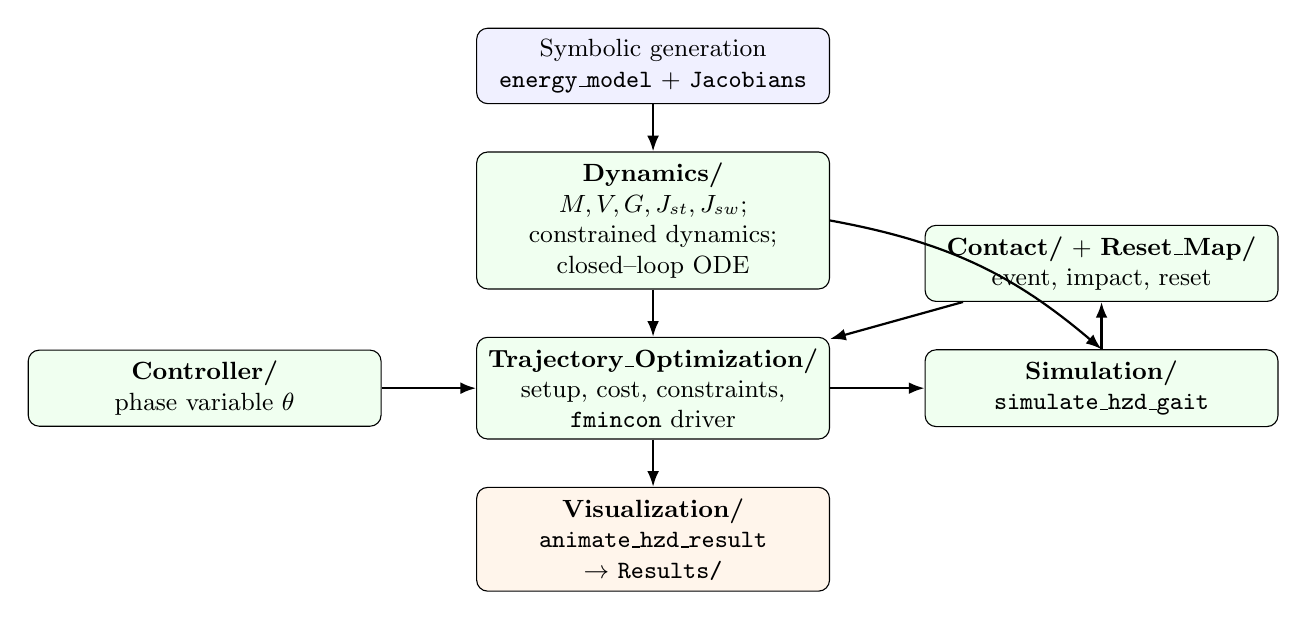
\begin{tikzpicture}[
    node distance=6mm and 12mm,
    box/.style={draw, rounded corners, align=center, inner sep=4pt,
                text width=42mm, font=\small},
    gen/.style={box, fill=blue!6},
    core/.style={box, fill=green!6},
    io/.style={box, fill=orange!8},
    arr/.style={-{Latex[length=2mm]}, thick},
  ]
  \node[gen]  (elm)  {Symbolic generation\\ \fname{energy\_model} + \fname{Jacobians}};
  \node[core, below=of elm] (dyn) {\textbf{Dynamics/}\\ $M,V,G,J_{st},J_{sw}$;\\ constrained dynamics;\\ closed--loop ODE};
  \node[core, below=of dyn] (opt) {\textbf{Trajectory\_Optimization/}\\ setup, cost, constraints,\\ \fname{fmincon} driver};
  \node[core, right=of opt] (sim) {\textbf{Simulation/}\\ \fname{simulate\_hzd\_gait}};
  \node[core, above=of sim] (hyb) {\textbf{Contact/} + \textbf{Reset\_Map/}\\ event, impact, reset};
  \node[core, left=of opt]  (phase) {\textbf{Controller/}\\ phase variable $\theta$};
  \node[io, below=of opt] (viz) {\textbf{Visualization/}\\ \fname{animate\_hzd\_result}\\ $\rightarrow$ \fname{Results/}};

  \draw[arr] (elm) -- (dyn);
  \draw[arr] (dyn) -- (opt);
  \draw[arr] (phase) -- (opt);
  \draw[arr] (opt) -- (sim);
  \draw[arr] (sim) -- (hyb);
  \draw[arr] (hyb) -- (opt);
  \draw[arr] (dyn.east) to[bend left=15] (sim.north);
  \draw[arr] (opt) -- (viz);
\end{tikzpicture}
\caption{Pipeline: offline symbolic generation feeds the \textbf{Dynamics}
layer; the optimizer repeatedly calls the single--step simulator (which
integrates the closed--loop dynamics and detects impact) to evaluate the cost
and constraints; the converged gait is animated and saved.}
\end{figure}

% =====================================================================
\section{File reference}
% =====================================================================
\renewcommand{\arraystretch}{1.15}

\subsection*{Dynamics/ (mostly Symbolic--Toolbox generated)}
\begin{longtable}{@{}L{4.7cm} L{9.5cm}@{}}
\toprule
file & role \\
\midrule
\endhead
\fname{rabbit\_energy\_model\_generalized\_Lagrange.m} & Generator: Euler--Lagrange derivation; defines masses/inertias; produces \code{Tt,T1--T4,P\_st,P\_sw,M,DM,V,G}. \\
\fname{Jacobians.m} & Generator: produces \code{J\_st,J\_sw,Jdotdq\_st,Jdotdq\_sw}. \\
\fname{Tt.m}, \fname{T1--T4.m} & Homogeneous transforms of torso / link frames, \code{T=Tt(q)}. \\
\fname{P\_st.m}, \fname{P\_sw.m} & Stance / swing foot position $[x;z]$, world frame. \\
\fname{M.m} & Mass matrix $M(q)$ ($7\times7$). \\
\fname{V.m} & Coriolis/centrifugal vector, \code{V([q;dq])}. \\
\fname{G.m} & Gravity vector $G(q)$. \\
\fname{DM.m} & $\dot M$, \code{DM([q;dq])} (used to form $V$). \\
\fname{J\_st.m}, \fname{J\_sw.m} & Foot Jacobians ($2\times7$). \\
\fname{Jdotdq\_st.m}, \fname{Jdotdq\_sw.m} & $\dot J\dot q$ terms ($2\times1$). \\
\fname{input\_matrix.m} & Constant actuation map $B$. \\
\fname{rabbit\_constrained\_dynamics.m} & Single--support forward dynamics (KKT solve), \code{[ddq,lambda]=...(q,dq,u)}. \\
\fname{hzd\_closed\_loop\_ode.m} & Closed--loop swing RHS (B--spline + PD), augmented cost state. \\
\fname{rabbit\_ode.m} & Generic single--support RHS for an arbitrary controller. \\
\warn{rabbit\_dynamics.m} & \warn{Broken}: calls nonexistent \code{D\_matrix/C\_vector/G\_vector}. \\
\bottomrule
\end{longtable}

\subsection*{Contact/ and Reset\_Map/}
\begin{longtable}{@{}L{4.7cm} L{9.5cm}@{}}
\toprule file & role \\ \midrule \endhead
\fname{rabbit\_impact\_event.m} & ODE event: swing foot reaches ground. \\
\fname{impact\_event\_wrapper.m} & Same event for the augmented HZD state $\xi$. \\
\fname{rabbit\_impact\_map.m} & Momentum--conserving velocity reset, \code{x\_plus=...(x\_minus)}. \\
\fname{relabel\_state.m} & Swap stance/swing joints and velocities. \\
\fname{rabbit\_reset\_map.m} & Relabel + re--plant stance foot on ground. \\
\bottomrule
\end{longtable}

\subsection*{Controller/}
\begin{longtable}{@{}L{4.7cm} L{9.5cm}@{}}
\toprule file & role \\ \midrule \endhead
\fname{theta\_of\_q.m} & Phase variable $\theta=q_t+q_1+\tfrac12 q_2$. \\
\fname{dtheta\_dq\_of.m} & Constant gradient $c$. \\
\warn{rabbit\_controller.m} & \warn{Broken}: calls nonexistent \code{desired\_gait}. \\
\bottomrule
\end{longtable}

\subsection*{Trajectory\_Optimization/ (main pipeline)}
\begin{longtable}{@{}L{4.7cm} L{9.5cm}@{}}
\toprule file & role \\ \midrule \endhead
\fname{rabbit\_hzd\_trajectory\_optimization.m} & \textbf{Entry point}: single--gait solve, save, animate. \\
\fname{build\_gait\_library.m} & Speed continuation; builds a \code{gait\_library} struct. \\
\fname{hzd\_problem\_setup.m} & Single source of $p$, bounds, \code{fmincon} options. \\
\fname{hzd\_cost.m} & Objective (torque$^2$ per step length). \\
\fname{hzd\_constraints.m} & Equality + inequality constraints. \\
\fname{unpack\_z.m} & Split $z=[\text{coeffs};x_{\text{start}}]$. \\
\fname{make\_coeffs.m} & Initial B--spline control points. \\
\fname{bspline\_eval.m} & Evaluate a spline output and its $s$--derivative. \\
\fname{BSpline.m}, \fname{BSpline\_derivative.m} & Cox--de Boor basis and derivative. \\
\fname{inspect\_solution.m} & Full diagnostic breakdown of a solution (incl. $\rho$). \\
\fname{poincare\_stability.m} & Step--map Jacobian; returns spectral radius $\rho$ (NEC5). \\
\fname{settle\_initial\_state.m} & Poincar\'e iteration (disabled by default). \\
\bottomrule
\end{longtable}

\subsection*{Simulation/, Utilities/, Visualization/}
\begin{longtable}{@{}L{4.7cm} L{9.5cm}@{}}
\toprule file & role \\ \midrule \endhead
\fname{simulate\_hzd\_gait.m} & One HZD step, summary outputs (status, penetration, clearance, $T_{\text{step}}$). \\
\fname{simulate\_hzd\_gait\_full.m} & One HZD step, full trajectory (for animation/drift). \\
\fname{simulate\_one\_step.m} & Generic one step for an arbitrary controller. \\
\fname{simulate\_n\_steps.m} & Chain generic steps with impact+reset. \\
\fname{get\_body\_points.m} & World positions of key body points. \\
\fname{check\_ground\_validity.m} & Ground/penetration/slip validation of a state. \\
\fname{animate\_rabbit.m} & Stick--figure animation + GIF export. \\
\fname{animate\_hzd\_result.m} & Stitch $n$ HZD steps and animate. \\
\bottomrule
\end{longtable}

\subsection*{config/ and Test/}
\begin{longtable}{@{}L{4.7cm} L{9.5cm}@{}}
\toprule file & role \\ \midrule \endhead
\fname{make\_initial\_state.m} & Deterministic ground--valid start state (1 output). \\
\fname{make\_random\_initial\_state.m} & Rejection--sampled random start (unseeded). \\
\fname{config.m} & Singleton: stepping--stone terrain + spline params. \\
\fname{init\_bspline\_params.m} & Legacy B--spline controller config. \\
\fname{test\_simulate\_steps.m} & Smoke test of the generic simulation path. \\
\bottomrule
\end{longtable}

% =====================================================================
\section{Reproducibility}
% =====================================================================
\begin{itemize}
  \item \textbf{Generated dynamics.} \code{Tt,T1--T4,P\_st,P\_sw,M,DM,V,G} come
        from \fname{rabbit\_energy\_model\_generalized\_Lagrange.m};
        \code{J\_st,J\_sw,Jdotdq\_st,Jdotdq\_sw} from \fname{Jacobians.m}.
        \emph{If any mass, length, inertia, or kinematic relation changes, these
        generator scripts must be re--run} to regenerate the committed files.
        Do not hand--edit the generated files.
  \item \textbf{Saved results.} \fname{Results/hzd\_result\_<timestamp>.mat}
        each store \code{z\_opt, p, fval, exitflag, report}. The
        \code{2026-07-20\_12-06-36} result is the reference periodic gait
        ($\approx 0.355\,$m/s) used as the warm--start seed.
        \fname{build\_gait\_library.m} writes
        \fname{gait\_library\_<timestamp>.mat}.
  \item \textbf{Nondeterminism.} \fname{make\_random\_initial\_state.m} uses
        \code{randn} with no seed. The HZD pipeline instead uses a hard--coded
        $x_0$, so its results are reproducible. Add \code{rng(seed)} before
        random sampling if determinism is needed there.
  \item \textbf{Orphaned cache.} \fname{Trajectory\_Optimization/Trajectory.mat}
        is committed but loaded by no code path; treat as unverified.
  \item \textbf{Simscape.} \fname{Dynamics/Test\_dynamics\_Simscape.slx} is a
        standalone dynamics cross--check, not part of the runtime pipeline.
\end{itemize}

% =====================================================================
\section{Known issues and broken legacy entry points}
\label{sec:known}
% =====================================================================
The following predate the HZD pipeline and \warn{do not run as--is} --- they
call functions that no longer exist. They are retained for reference only.
\begin{itemize}
  \item \fname{main\_demo.m}: calls \code{make\_initial\_state} expecting 3
        outputs (it returns 1), \code{simulate\_n\_steps} with 4 arguments (it
        takes 3), and \code{animate\_rabbit\_stepping\_stones} (does not exist).
  \item \fname{Controller/rabbit\_controller.m}: calls \code{desired\_gait} /
        \code{desired\_gait\_velocity} (do not exist).
  \item \fname{Dynamics/rabbit\_dynamics.m}: calls \code{D\_matrix} /
        \code{C\_vector} / \code{G\_vector} (do not exist; the real terms are
        \code{M} / \code{V} / \code{G}).
\end{itemize}

\paragraph{Open item: stance--foot constraint drift (a symptom).}
The stance foot is held only by the acceleration--level contact constraint, so
\code{ode45} permits numerical drift of the foot within a step
($\sim 0.1$--$0.3$~m; \fname{inspect\_solution.m} reports it). The natural fix
is Baumgarte stabilization (\fname{rabbit\_constrained\_dynamics.m} supports it
via an optional \code{foot\_ref}), but on the reference gait it \emph{diverged}
rather than helping. That is not a flaw in Baumgarte: as
Section~\ref{sec:stability} shows, the seed orbit has $\rho\approx 3$, so it
amplifies the very corrections Baumgarte injects. The drift is thus best read as
\emph{another symptom of orbital instability}; enforcing $\rho<1$ addresses the
root cause, after which constraint stabilization becomes well behaved.

\paragraph{Open item: enforcing stability is expensive.}
The $\rho<1$ constraint is finite--difference heavy (Section~\ref{sec:stability}).
It is usable as a warm--started final phase but slow for a from--scratch solve; a
reduced (2--dimensional hybrid zero dynamics) stability condition, or an
analytic Poincar\'e Jacobian, would make it cheap. This is the natural next step
for the pipeline, alongside the CLF--QP controller route (which stabilizes an
open--loop--unstable orbit with feedback instead of redesigning it).

% =====================================================================
\section*{References}
% =====================================================================
\begin{enumerate}
  \item E.~R.~Westervelt, J.~W.~Grizzle, C.~Chevallereau, J.~H.~Choi, B.~Morris,
        \emph{Feedback Control of Dynamic Bipedal Robot Locomotion},
        CRC Press, 2007.
\end{enumerate}

\end{document}
